\chapter{Résultats}


\paragraph{Performance théorique:} Suite à l'apprentissage du réseau de neurone, nous avons obtenu une précision de 59.0\% sur les données d'entrainement,
de 58.9\% sur les données de tests avant quantization et 58\% après.
La matrice de confusion nous permet de voir que les chants ont été globalement 
bien appris avec une majorité de vrais positifs pour la plupart des classes cf: Figure \ref{graph:confusion_matrix1}.
Les classes présentant le plus de confusion sont les classes 0, 3, 4 et 5 avec un maximum de confusion pour la classe 3.
Ces classes représentent les oiseaux suivants :

\begin{itemize}
  \item 0: Alauda Arvensis
  \item 3: Emberiza Cirlus
  \item 4: Emberiza Citrinella
  \item 5: Falco Tinnunculus
\end{itemize}

\begin{figure}[!ht]
  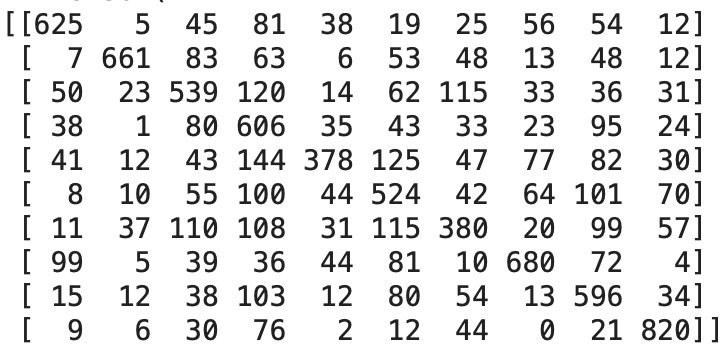
\includegraphics[width=0.5\textwidth]{confusion_matrix1}
  \centering
  \caption{Matrice de confusion}
  \label{graph:confusion_matrix1}
\end{figure}

\paragraph{Performance expérimentale:} Pour tester nos résultats nous avons déployé le réseau de neurone sur la carte Nucleo à l'aide 
de l'IDE Arduino. Pour cela nous avons utilisé le même projet Arduino que dans le Lab 5, lors de la réalisation du CNN à partir du
jeu de donnée Google Speech Commons. Nous avons modifié le programme pour qu'il n'écrive dans la sortie Serial que lorsque la valeur prédite maximum
est supérieure à 8000. Cela permet le n'afficher que les résultats ou ceux-ci sont plus en faveur d'une classe que d'une autre.
Nous avons ensuite testé de modèle en jouant sur haut-parleur des sons n'étant pas présents dans notre jeu de données.

Nous avons pu remarquer que lorsque qu'un chant d'oiseau est joué et qu'un résultat est donné, celui-ci est le bon dans la majorité des cas.
Cependant, nous recevons parfois des résultats en présence de bruits forts, alors qu'aucun bruit d'oiseau n'est joué. 
Cela peut être dû à la présence dans notre jeu de données d'échantillons de bruits de fond, où aucun oiseau ne peut être entendu.

\paragraph{Mémoire:} Pour évaluer la mémoire utilisée par la carte, nous avons utilisé Arduino en mode verbose pour pouvoir 
lire la ROM puis nous avons utilisé la dernière commande exécutée pour accéder au fichier elf et estimer la RAM.

\begin{figure}[!ht]
  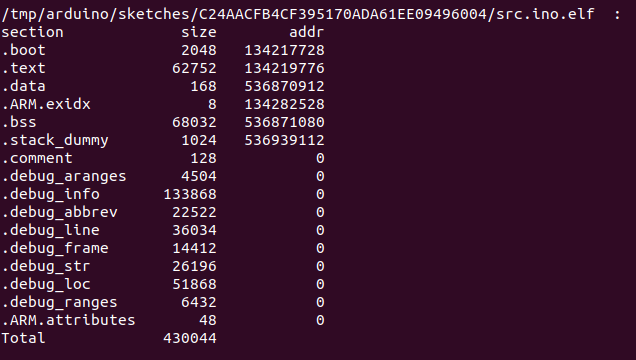
\includegraphics[width=0.5\textwidth]{elf}
  \centering
  \caption{Contenu du fichier elf}
  \label{graph:confusion_matrix1}
\end{figure}

\begin{center}
  \begin{tabular}{|c|c|}
   \hline
    ROM & 64 968 octets\\
   \hline
    RAM & 68 032 octets\\
   \hline
  \end{tabular}
\end{center}

\paragraph{Latence: } Nous n'avons pas pu tester la latence de la carte à l'aide du script d'évaluation python. 
Nous considérons donc que celle-ci est de 60 ms.
\paragraph{Energie: } La carte utilisée étant la même que celle de la RFThings-AI Dev Kit board, nous faisons 
supposons que la consommation en mode active est la même (62 mW) et que la consommation en mode veille est nulle. 
Nous supposons également que l'appareil collectera des données sur une durée de 2,56 secondes.
Enfin, nous considérons que la carte utilisera deux piles de type AA Alcalines ayant une charge de 3900 mWh.

\begin{center}
  \begin{tabular}{|c|c|c|}
   \hline
     & Unité de mesure & Estimation\\
   \hline
    \makecell{Consommation énergétique \\ en mode actif} & mW & 62\\
   \hline
    \makecell{Consommation énergétique \\ moyenne par inférence} & mW & $62*\frac{0.06}{2.56} = 1.453$\\
   \hline
    \makecell{Énergie de batterie} & mW & 7 800\\
   \hline
    \makecell{Autonomie de l'appareil \\ avec mode veille} & h & $\frac{7800}{1.453} = 5368$\\
   \hline
    \makecell{Autonomie de l'appareil \\ sans mode veille} & h & $\frac{7800}{62} = 126$\\
   \hline
  \end{tabular}
\end{center}
